\chapter{Introduction}
\label{chap:introduction}

Facial animation is an important discipline in computer animation,
as faces convey a significant part of human expression or emotion.
This makes good facial animation an essential requirement for character animation in film or video games.
At the same time, animation efficiency can't be disregarded completely for high-quality results,
so an approach combining both model quality and model usability is desired.
\textit{Inverse kinematics} provides such an approach,
as it enables direct manipulation of high-quality blend shape models or performance driven facial animation using motion capture.

\section{Facial Animation Overview}
\label{sec:facialanimationmethods}

The simplest approach to facial animation could possibly be freeform deformation mixed with keyframe animation,
which allows to recreate any emotion or expression at the cost of labor intensity and missing \textquote{guardrails}:
This technique imposes no modeling restrictions, so unnatural facial deformations can be produced easily (see \autoref{fig:unnaturaldeformation}).

\begin{figure}[h]
  \centering
  \begin{subfigure}[b]{0.3\textwidth}
	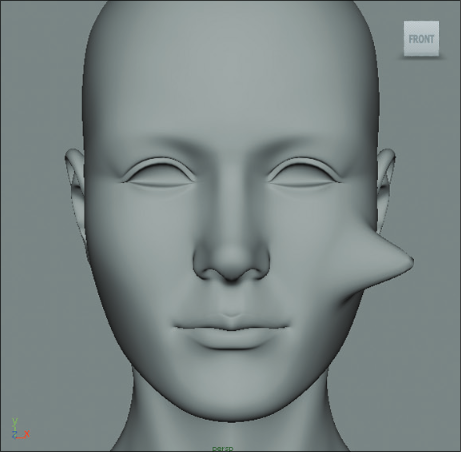
\includegraphics[scale=0.3]{img/unnatural_deformation.png}
  \end{subfigure}
  \caption{Unnatural Deformation.~\autocite{directmanipulationblendshapes}}
  \label{fig:unnaturaldeformation}
\end{figure}

To improve the model usability and prevent unnatural results,
the facial model can also be controlled through a set of parameters,
either chosen and implemented manually or automatically.

The (probably) first parametric face model was produced by F.I.\ Parke in 1974~\autocite{parametricface}:
It contains manually chosen parameters like \code{JAW ROTATION} (see \autoref{fig:parametricjawrotation}) or \code{MOUTH WIDTH} and applies different deformation operations like translation,
rotation or scaling on certain facial regions to realize them.

\begin{figure}[h]
  \centering
  \begin{subfigure}[b]{0.3\textwidth}
	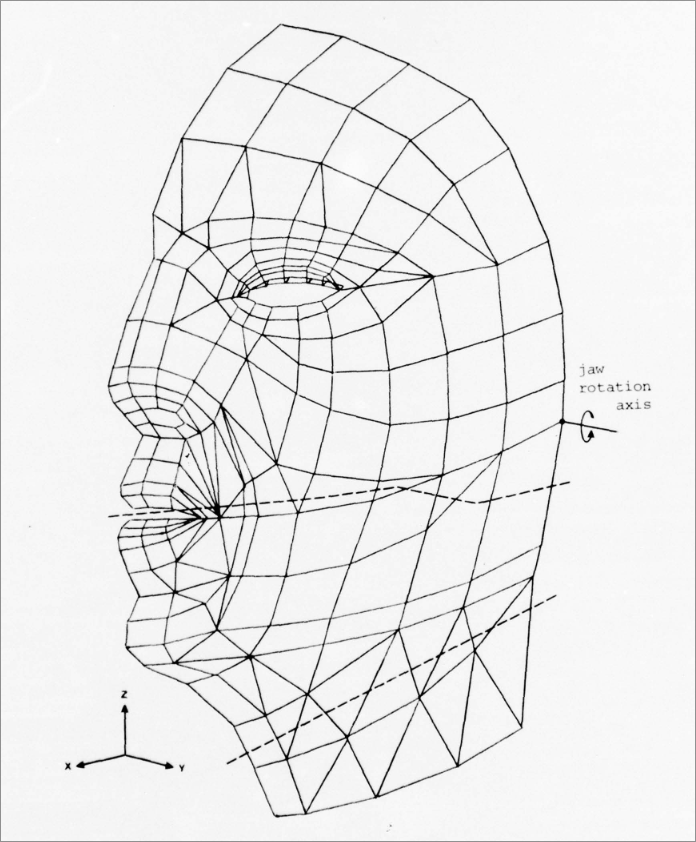
\includegraphics[scale=0.2]{img/parametric_model.png}
  \end{subfigure}
  \caption{Manually specified jaw rotation.~\autocite{parametricface}}
  \label{fig:parametricjawrotation}
\end{figure}

A different method to parameterize a face model is the \textquote{blend shape} approach:
Instead of using custom deformation operations on isolated parts of the mesh,
a blend shape model interpolates between different pre-modeled expressions that have identical vertex amounts and triangulation.
Multiple weighted expressions (\textquote{blend shape targets}) can be combined to generate the target expression.

By generating the target expression through a weighted sum of complete face models,
unwanted scale deformations can be introduced by choosing \textquote{wrong} weights.
Thus, the blend shape method was refined to combine local deviations from a neutral face instead,
called \textquote{delta blend shapes}.

Instead of manually associating each parameter with a certain expression,
model parameters can also be determined statistically,
e.g.\ by doing a principal component analysis of a range of facial expressions.
This generally results in non-interpretable model parameters,
which makes this model harder to animate,
as it is difficult to anticipate the resulting expression based on single parameter modifications.

It is also possible to apply more general character animation techniques like skeletal animation to faces,
as is often done in video games.
This approach is efficient to animate,
but weaknesses like unnatural skin and muscle movement become more significant in the case of faces,
so skeletal face animation might not be suitable if quality requirements are high.

Hybrid approaches,
like supplying a bone-driven model with a physical skin and muscle simulation,
can produce more realistic results,
but are also highly dependent on the character,
so the transfer of animations or \textquote{rigs} between characters might become difficult.
Also, physical simulation usually comes with a large performance impact,
which makes this technique unsuitable for real-time applications.

Skeletal rigs can also be combined with blend shapes,
as certain facial components that have a clear rotational axis (like eyes or jaw) are conveniently animated using a skeleton.
Blend shapes can then be used to correct skin movement or add detail.

\section{Kinematics}
\label{sec:kinematics}

Kinematics is a subfield of physics, dealing with the motion of bodies in a system while ignoring masses or forces.
A kinematic system in computer animation, like a skeleton, is modeled using rigid \textquote{bones} and rotatable \textquote{joints}\footnote{
  This differs for the blend shape approach,
  which is further described in \autoref{chap:blendshapemodels}.
}:

\begin{figure}[h]
  \centering
  \begin{subfigure}[b]{0.3\textwidth}
	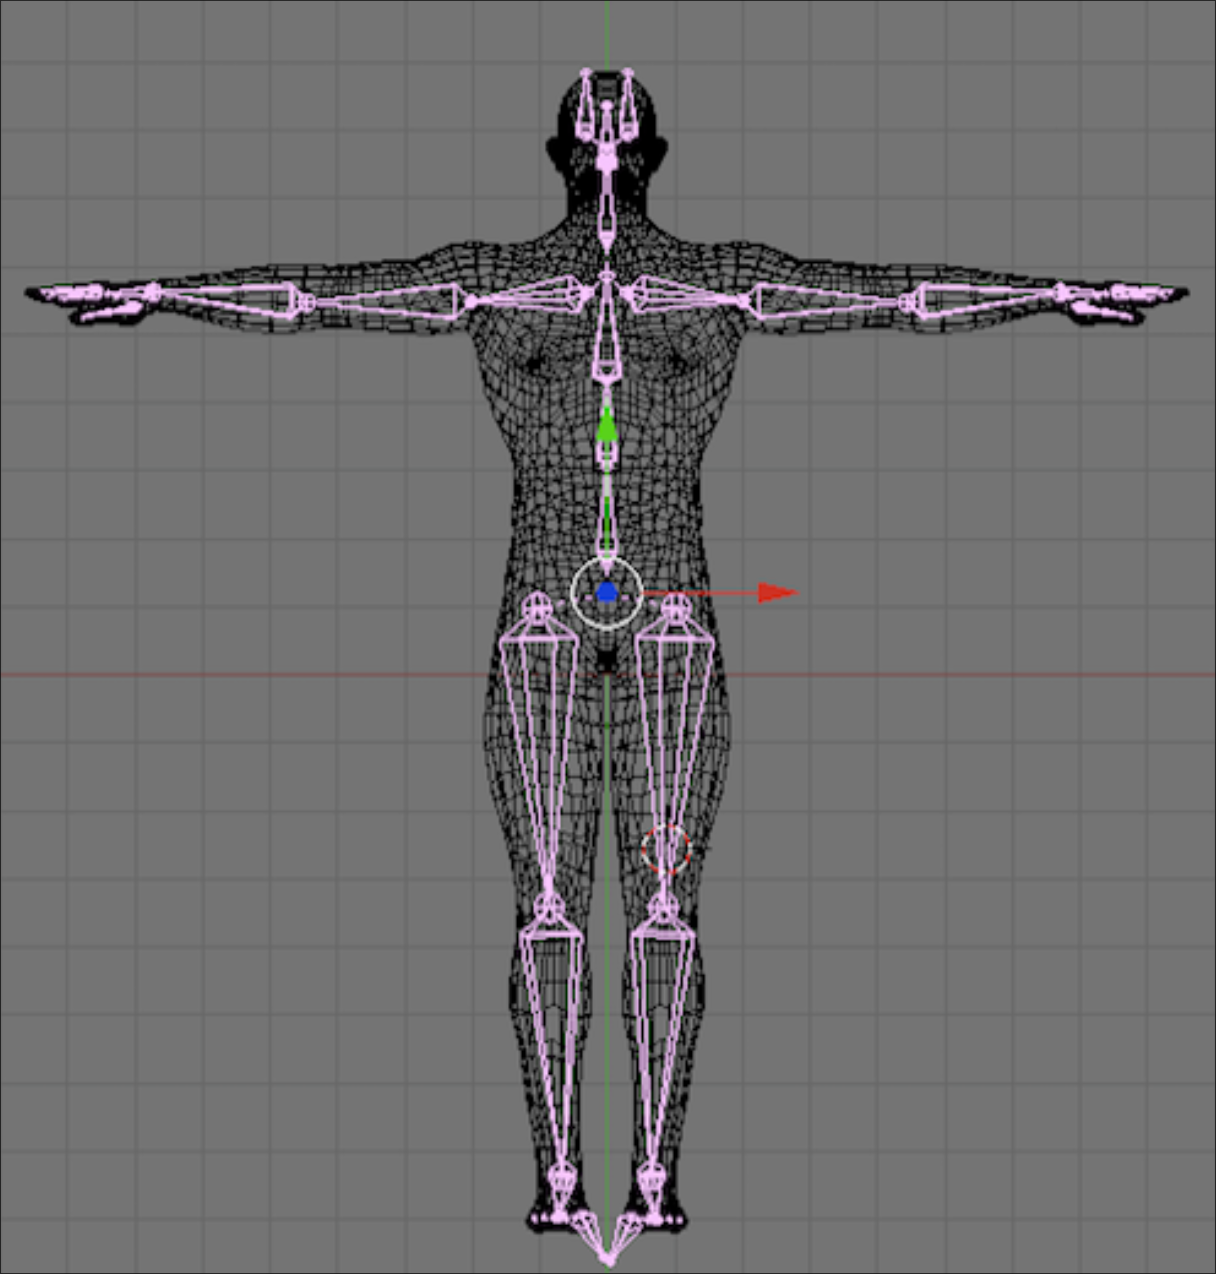
\includegraphics[scale=0.1]{img/human_rig.png}
  \end{subfigure}
  \caption{Human skeleton rig.~\autocite{computeranimation}}
  \label{fig:humanrig}
\end{figure}

The bones are ordered in a hierarchical relationship:
Rotating a single \textquote{parent} bone around its joint also rotates all \textquote{children} bones accordingly along the same center of rotation.
Controlling such a kinematic model can happen in two ways: Forward and inverse kinematics.

\textbf{Forward kinematics} calculates the absolute position of a joint (also called \textquote{end effector}) based on given joint orientations/angles of the parent joints.
In general, the forward kinematics problem can be expressed as \(x=f(\theta)\),
where \(x=(x_1,\dots,x_n)^T\) are the effector positions and \(\theta=(\theta_1,\dots,\theta_n)^T\) are the joint angles.

\textbf{Inverse kinematics} describes the opposite problem \(\theta=f^{-1}(x)\):
The absolute effector positions are given and the angles that produce these positions are to be determined.
Solving this problem for real-world models is difficult for multiple reasons:

\begin{itemize}
  \item High-quality kinematic models (e.g.\ for character animation) can have hundreds of degrees of freedom
  \item Multiple solutions or no solutions at all are possible
        (for a given \(x_2\) in \autoref{fig:2dforwardkinematics} there are two solutions for \(\theta\) already,
         as \(\theta_1\) and \(\theta_2\) can be exchanged)
  \item Different solutions can be ordered by criteria that are difficult to define analytically,
        for example by \textquote{intuitiveness} or if a solution is appropriate in the context of an animation
\end{itemize}

In consequence, approximative solvers are typically preferred over analytical ones.
